\subsection{Tìm kiếm ảnh}

Người dùng có thể tìm kiếm các ảnh trong hệ thống với các từ khóa khác nhau như tên album, tên ảnh, tên người dùng, hoặc các từ khóa khác liên quan đến ảnh. Giao diện tìm kiếm ảnh được thể hiện trong hình \ref{fig:search-screen}. 

\begin{figure}[H]
    \centering
    \begin{subfigure}{0.32\textwidth}
        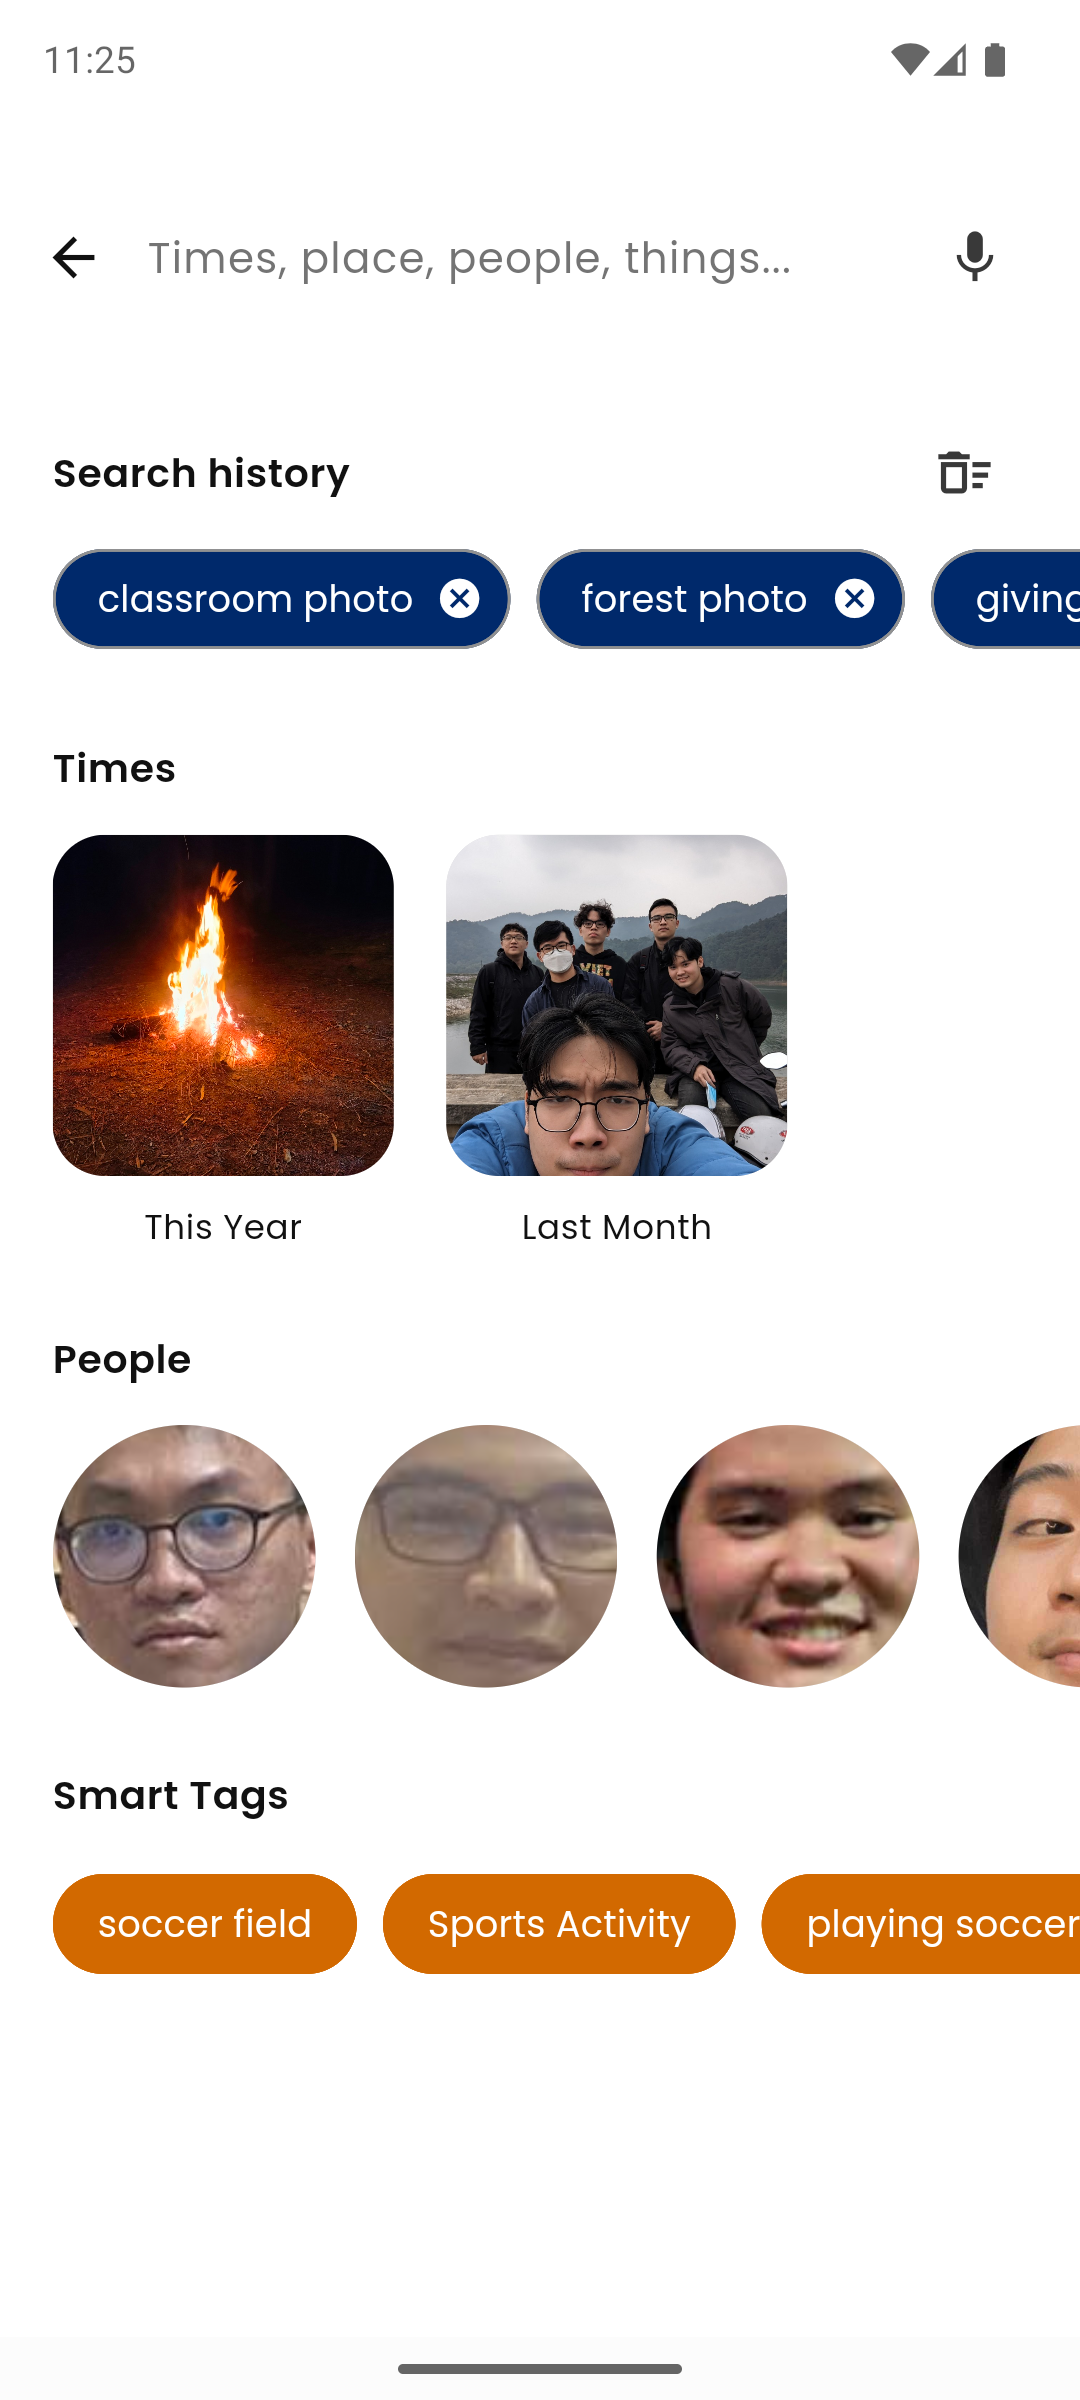
\includegraphics[width=1\linewidth]{figures/c4/4-2/search_1.png} 
        \caption{Các gợi ý tìm kiếm}
    \end{subfigure}
    \hfill
    \begin{subfigure}{0.32\textwidth}
        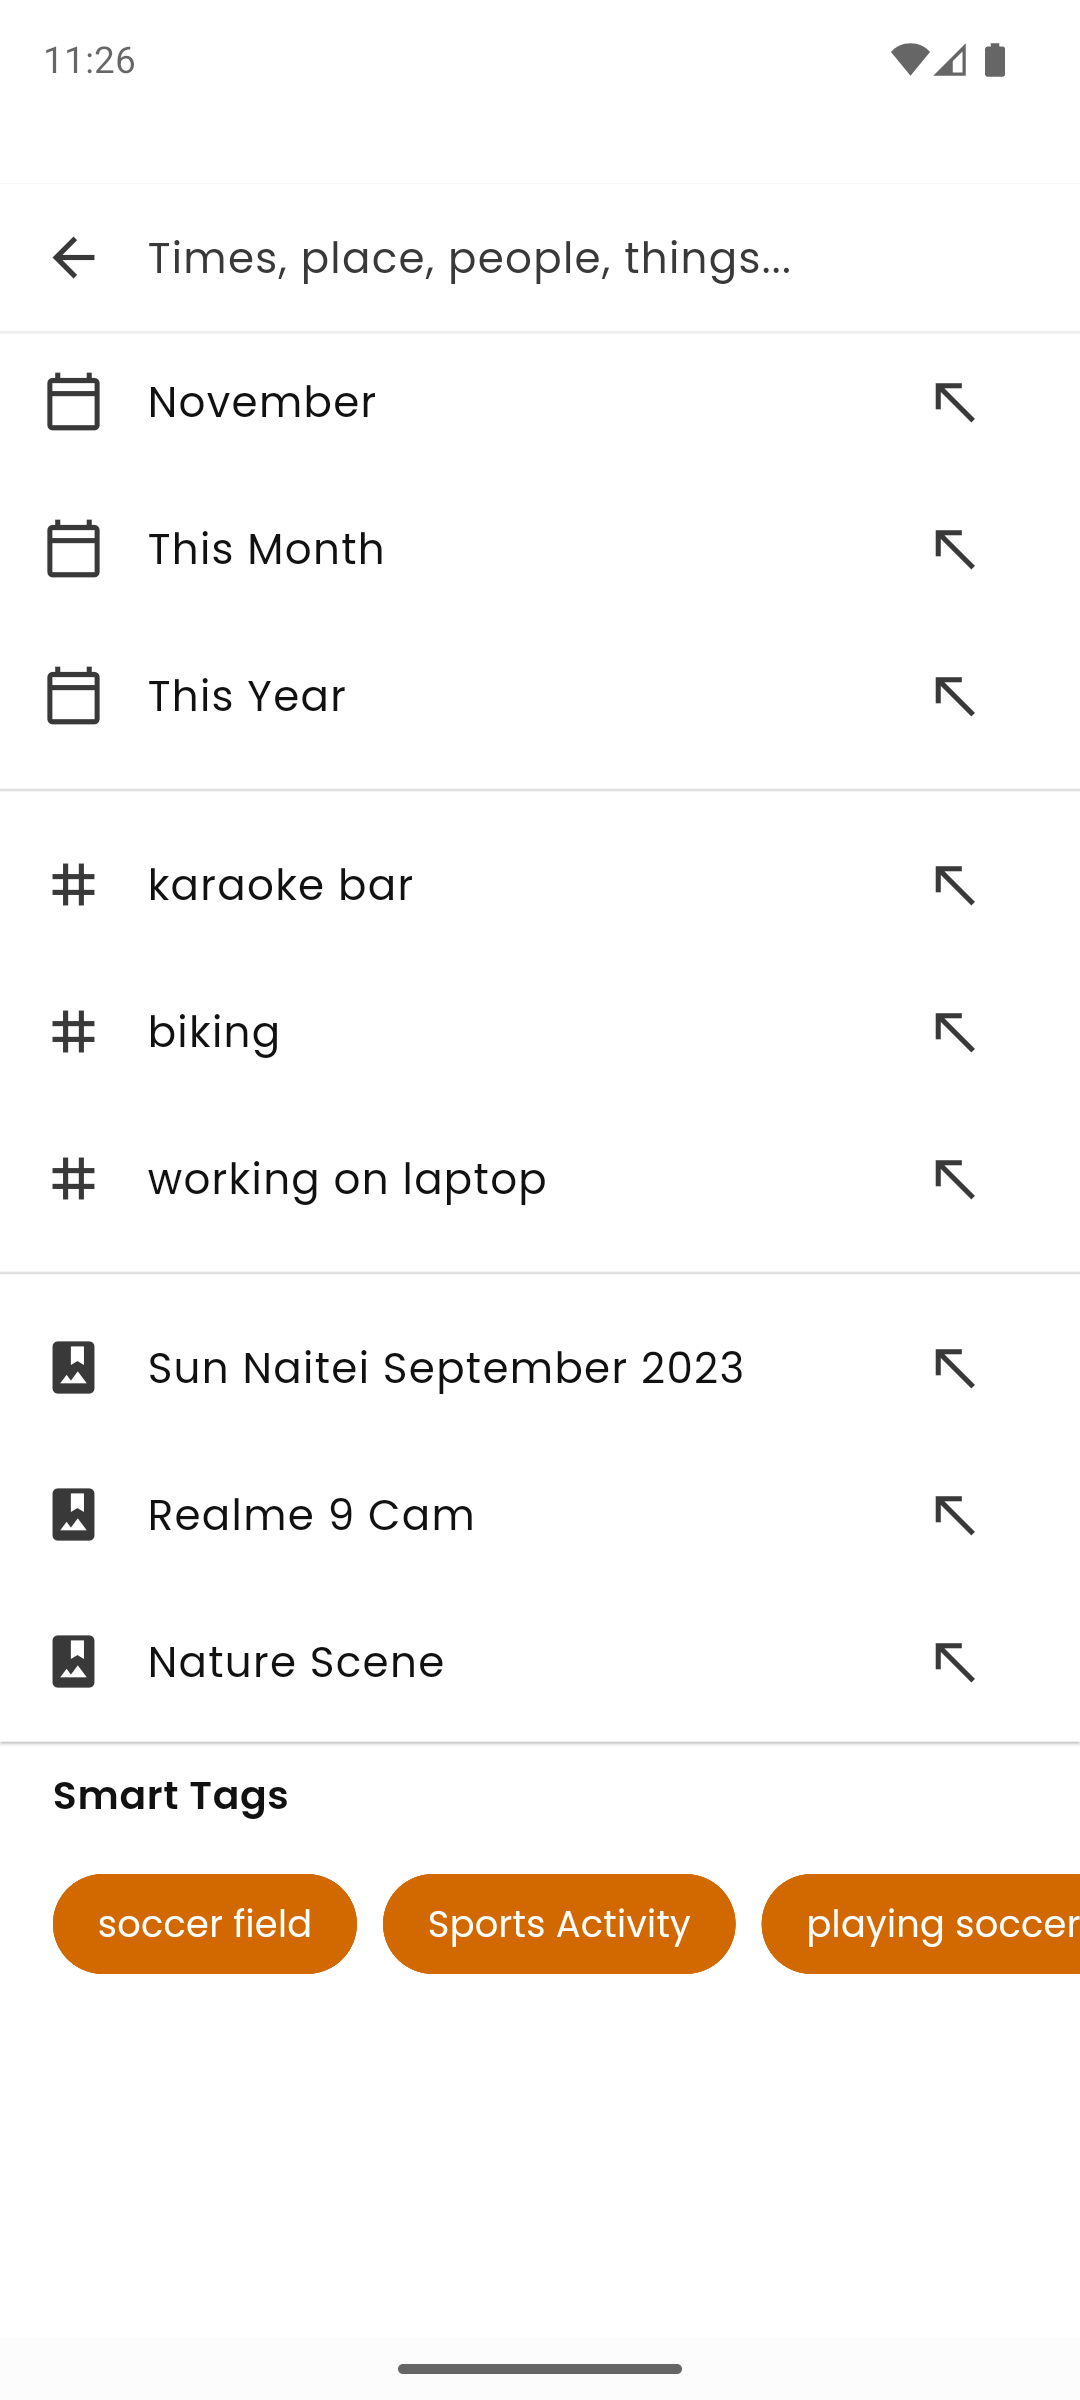
\includegraphics[width=1\linewidth]{figures/c4/4-2/search_2.png} 
        \caption{Gợi ý từ khóa tìm kiếm}
    \end{subfigure}
    \begin{subfigure}{0.32\textwidth}
        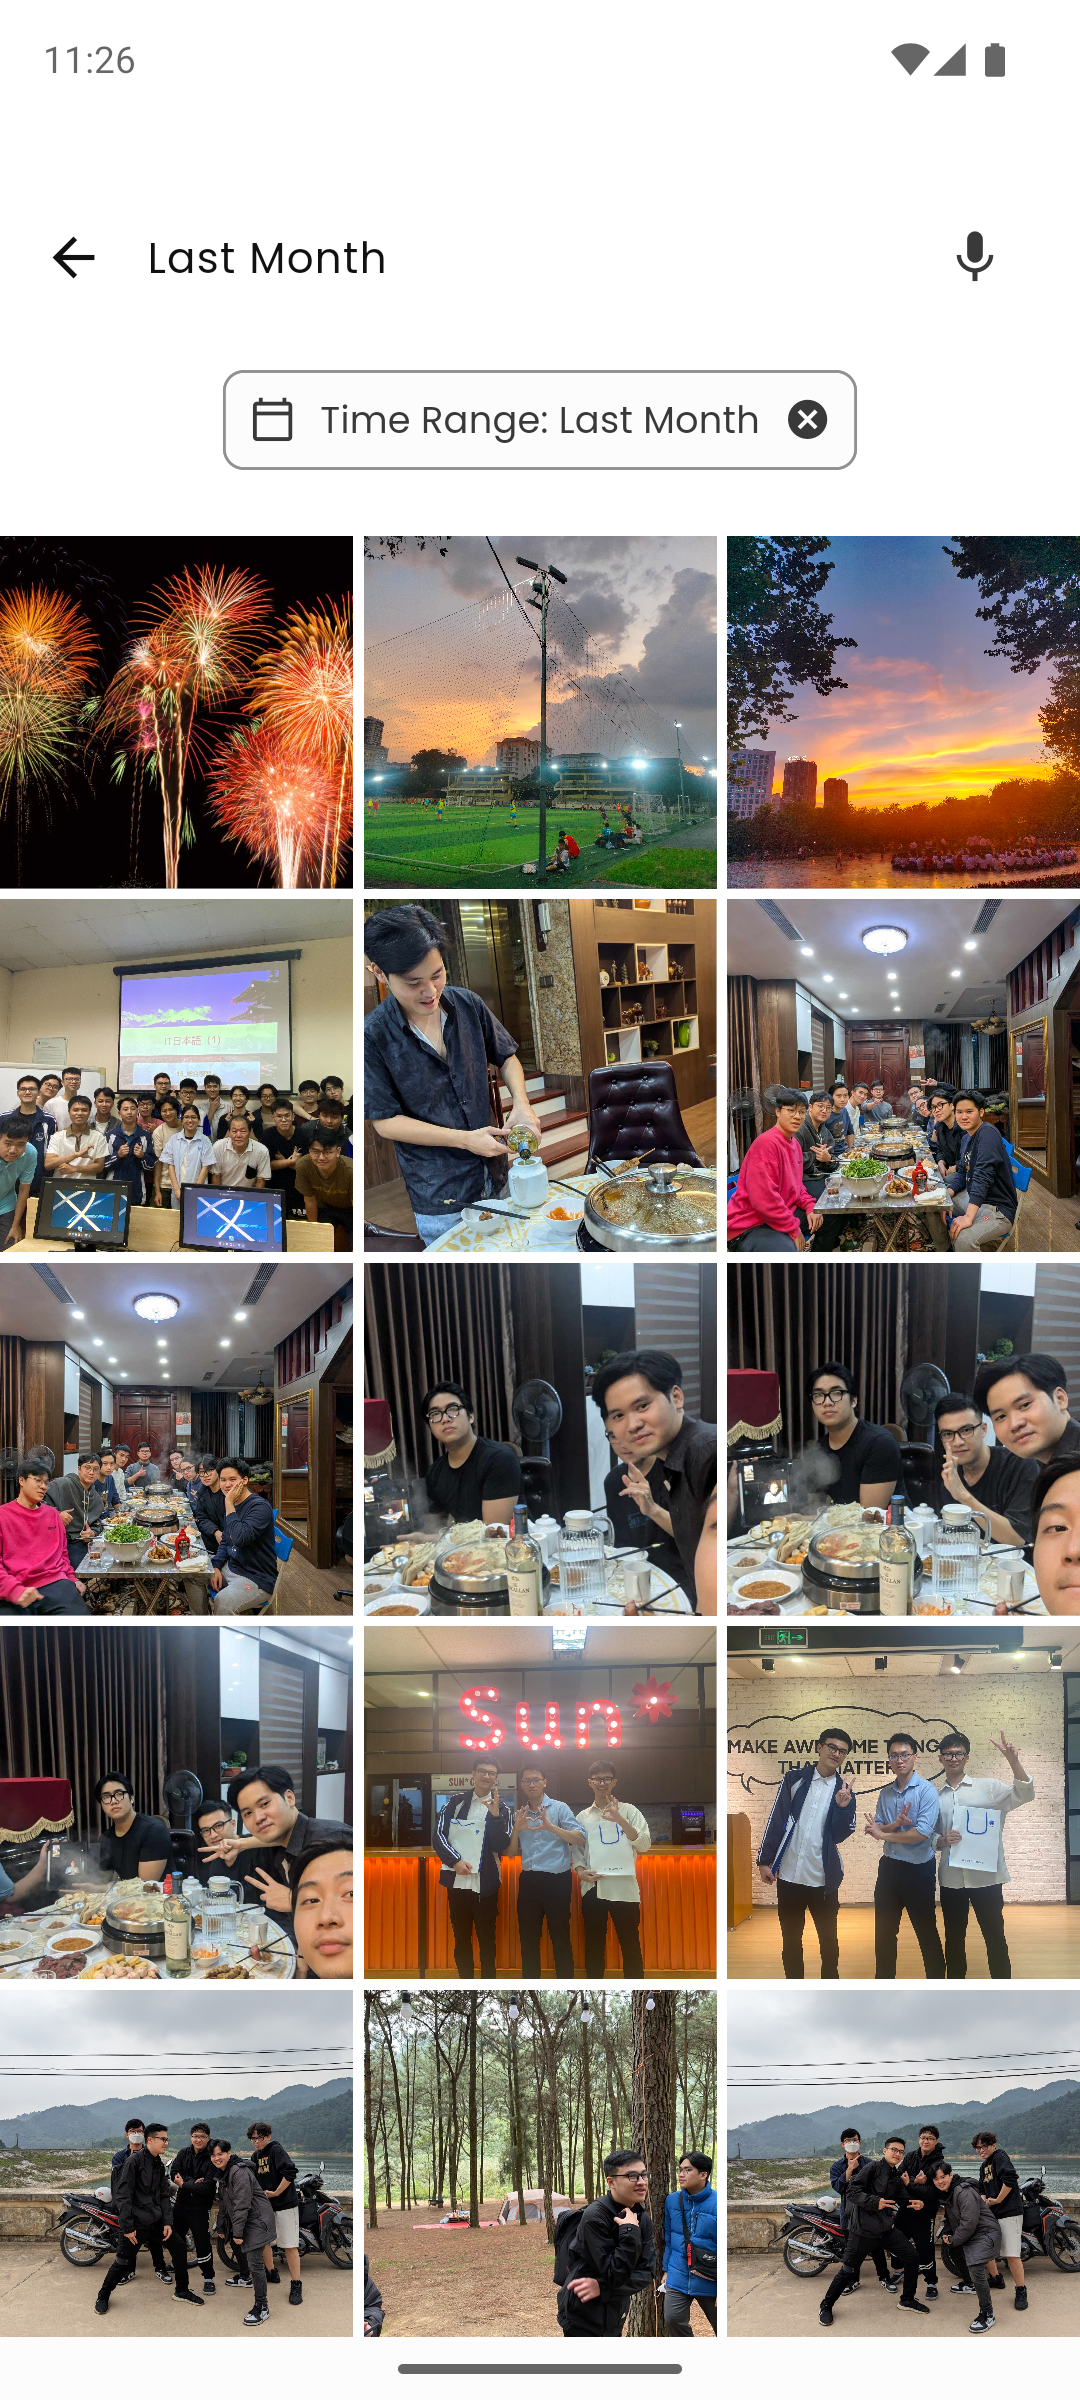
\includegraphics[width=1\linewidth]{figures/c4/4-2/search_4.png} 
        \caption{Kết quả tìm kiếm}
    \end{subfigure}
    \caption{Giao diện tìm kiếm.}
    \label{fig:search-screen}
\end{figure}

% Kết quả tìm kiếm sẽ được hiện thành danh sách và được sắp xếp theo thời gian tải lên. Ngoài ra hệ thống cũng cung cấp tính năng tìm kiếm ảnh bằng giọng nói. Giao diện kết quả tìm kiếm và tìm kiếm bằng giọng nói được thể hiện trong Hình \ref{fig:search-result}.

% \begin{figure}[H]
%     \centering
%     \begin{subfigure}{0.48\textwidth}
%         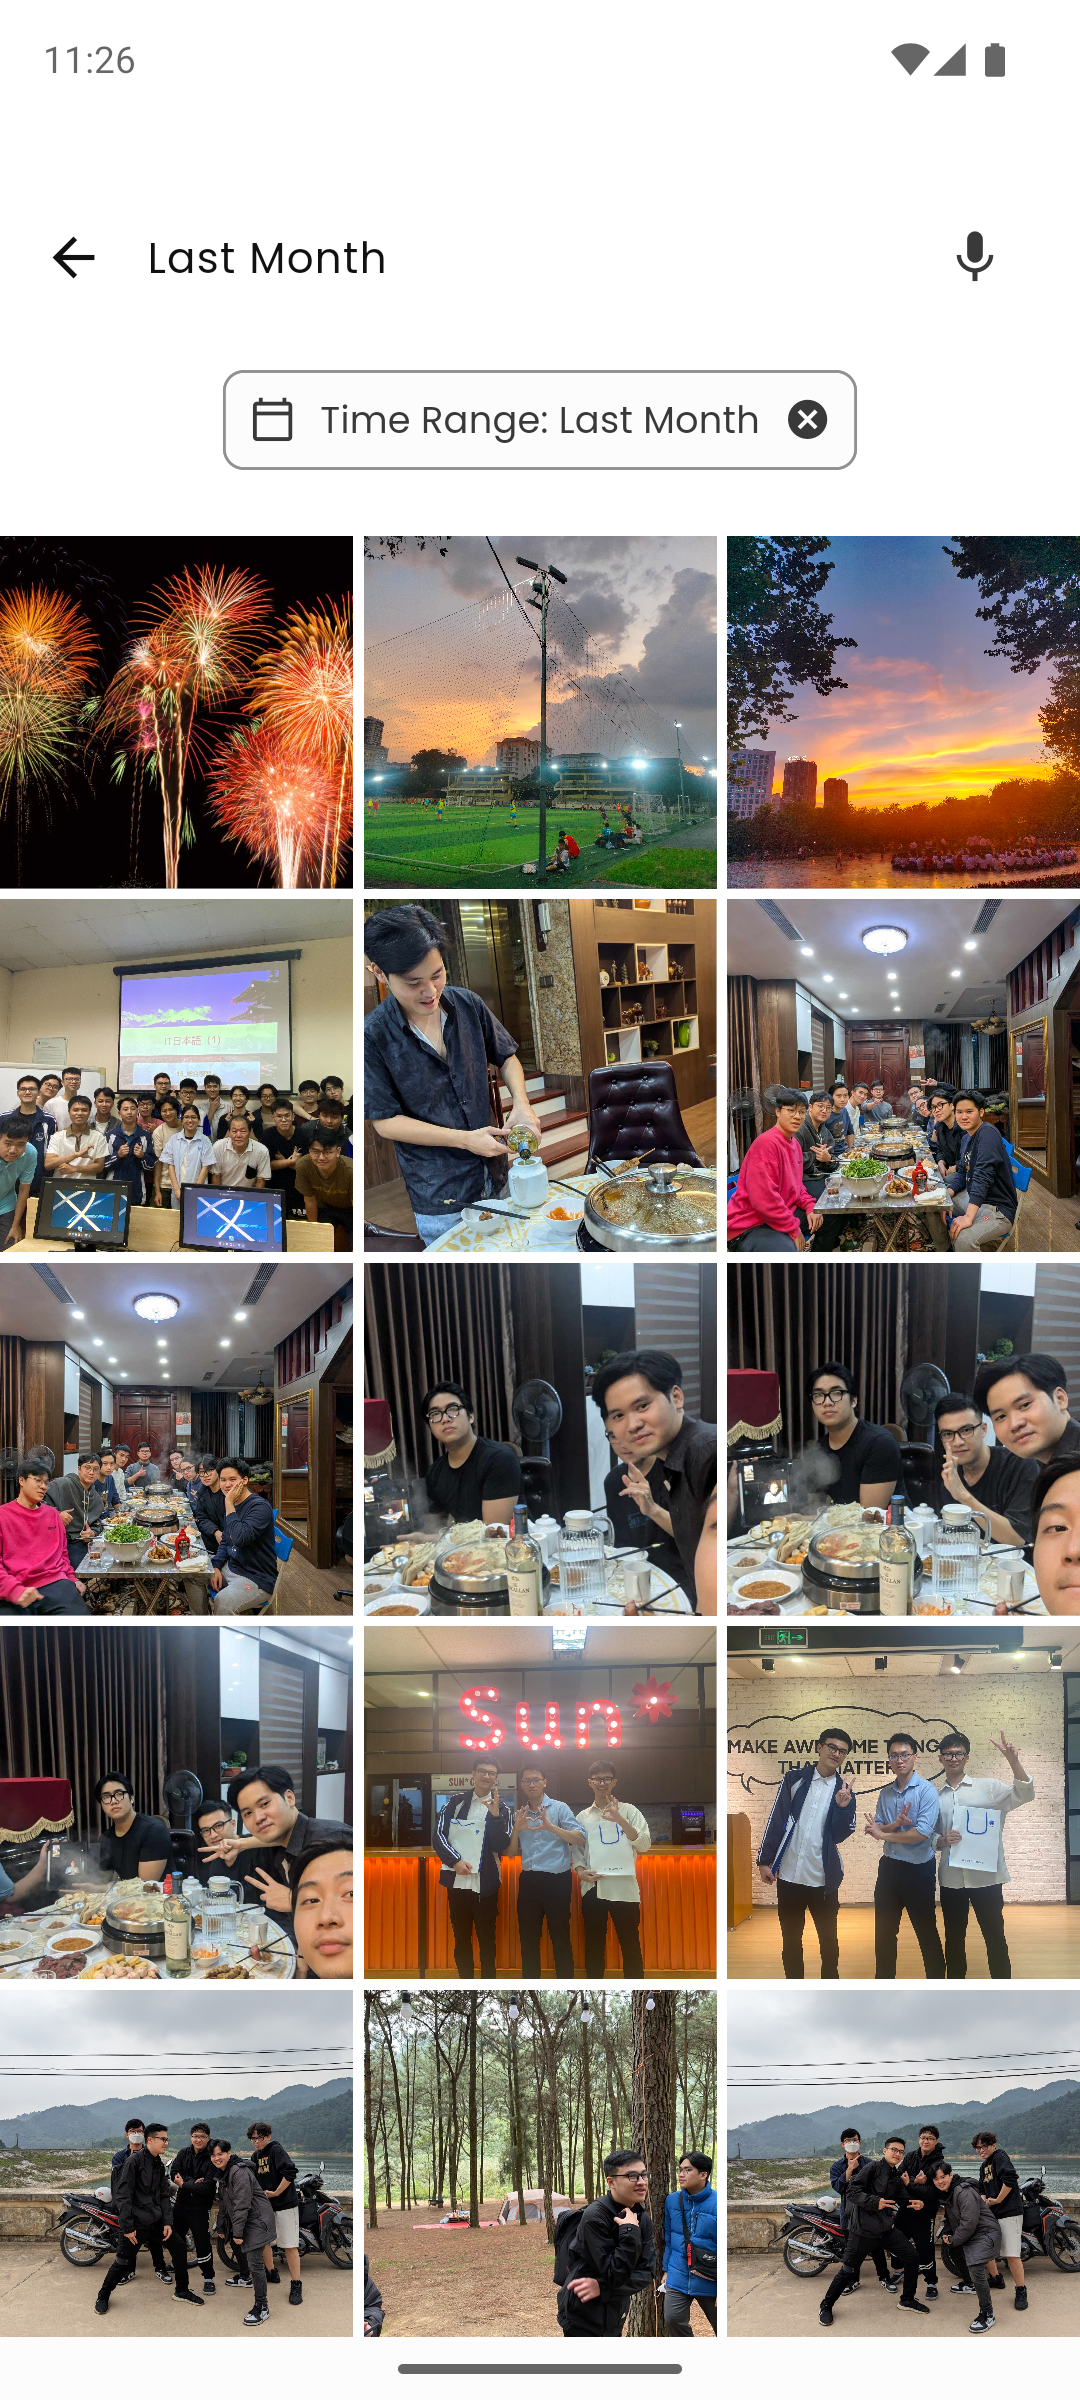
\includegraphics[width=1\linewidth]{figures/c4/4-2/search_4.png} 
%         \caption{Kết quả tìm kiếm}
%     \end{subfigure}
%     \hfill
%     \begin{subfigure}{0.48\textwidth}
%         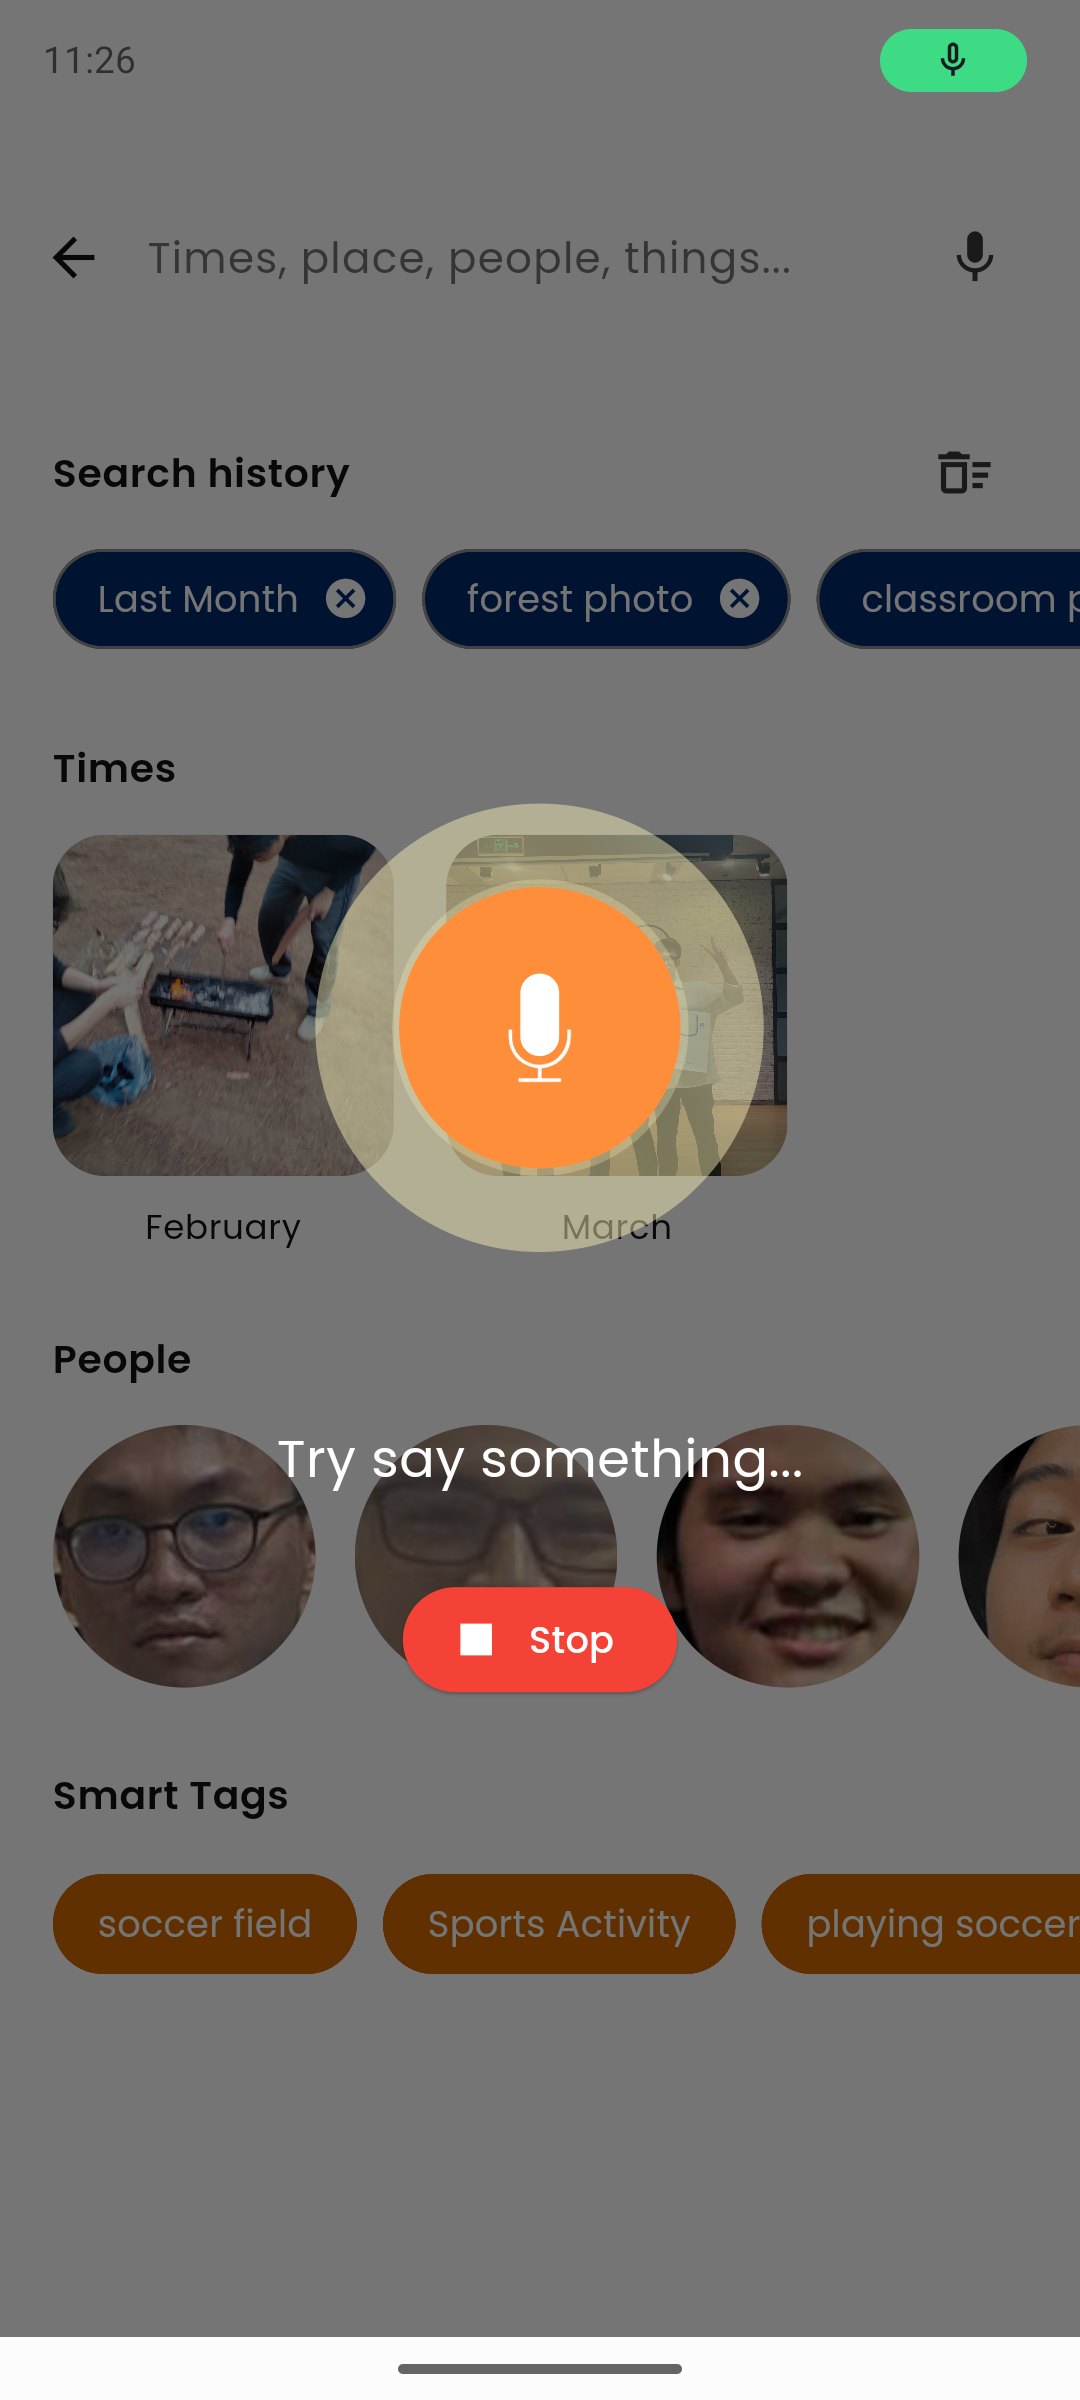
\includegraphics[width=1\linewidth]{figures/c4/4-2/search_3.png} 
%         \caption{Tìm kiếm bằng giọng nói}
%     \end{subfigure}
%     \caption{Giao diện tìm kiếm (2).}
%     \label{fig:search-result}
% \end{figure}